A continuacion, se describe el diseño detallado del sistema Thary, el cual consiste en las siguientes etapas del pipeline:

\paragraph{Etapa 1: Carga y limpieza de datos}
La primera etapa del pipeline (\texttt{app/services/prediccion/carga\_datos.py}) recibe el archivo CSV cargado por el administrador y lo normaliza hacia un esquema interno unico:


\begin{minted}{python}
ETIQUETAS_COLUMNAS_OBLIGATORIAS = {
    "fecha": "Fecha (o Date, Sale_Date)",
    "producto_id": "Producto (o Product, Product_ID)",
    "demanda": "Demanda (o Demand, Sales, Quantity_Sold)",
}


def cargar_y_limpiar(ruta_archivo):
    try:
        df = pd.read_csv(ruta_archivo)
    except pd.errors.EmptyDataError:
        raise ValueError("El archivo está vacío. Sube un CSV con al menos una fila de datos.")
    except pd.errors.ParserError:
        raise ValueError(
            "No se pudo leer el archivo como CSV. Verifica que sea un archivo de texto "
            "separado por comas (por ejemplo, no un Excel renombrado a .csv)."
        )
    except UnicodeDecodeError:
        raise ValueError(
            "El archivo tiene una codificación de caracteres que el sistema no reconoce. "
            "Guárdalo como CSV con codificación UTF-8 e intenta de nuevo."
        )

    if df.empty:
        raise ValueError("El archivo no tiene filas de datos, solo encabezados.")

    df = df.rename(columns={
        "Sale_Date": "fecha", "Date": "fecha", "date": "fecha", "Fecha": "fecha",
        "Product_ID": "producto_id", "Product": "producto_id", "Producto": "producto_id",
        "Quantity_Sold": "demanda", "Sales": "demanda", "Demand": "demanda", "Demanda": "demanda",
# ... variantes adicionales para precio, inventario, categoria, proveedor y lead time
    })

    columnas_faltantes = [c for c in ETIQUETAS_COLUMNAS_OBLIGATORIAS if c not in df.columns]
    if columnas_faltantes:
        faltan = ", ".join(ETIQUETAS_COLUMNAS_OBLIGATORIAS[c] for c in columnas_faltantes)
        raise ValueError(
            f"Al archivo le falta al menos una columna obligatoria: {faltan}. "
            "Agrégala al CSV (con ese nombre exacto u otro de los aceptados) y vuelve a subirlo."
        )
\end{minted}

En esta sección del archivo (\texttt{app/services/prediccion/carga\_datos.py}), se observa la etapa de carga y limpieza de los datos. Para garantizar que el sistema pueda adaptarse y funcionar para todo tipo de dominio de inventarios, se normalizan los nombres de las columnas de los archivos CSV con el fin de mantener un esquema más heterogéneo, de manera que el sistema pueda aceptar archivos de distintos dominios sin tener la necesidad de modificar el resto del pipeline. Para facilitarle al usuario el proceso de cargar un archivo, se capturan los errores mas comunes para el sistema a la hora de leer un CSV y se muestran a manera de mensaje de error en un lenguaje sencillo y facil de entender.

Otra practica que fue aplicada es el manejo de errores con mensajes dirigidos al usuario final, de esta manera, se evita que se propaguen los errores internos del sistema y el usuario sabe que es lo que esta ocurriendo y que es lo que se debe hacer para resolverlo.


\paragraph{Etapa 2: Segmentación de productos}
La segunda etapa del pipeline (\texttt{app/services/prediccion/segmentacion.py}) se basa en poder clasificar cada producto segun dos criterios principales:

\begin{itemize}
    \item Clasificacion ABC: Esta clasificacion permite poder identificar cual es la importancia relativa de cada producto dentro de la demanda total. Se calcula ordenando los productos de mayor a menor en base a su demanda total y se guarda su porcentaje. 
    
    Los productos que en conjunto representan hasta el 80\% de la demanda, se clasifican como categoria A, es decir, los mas importantes. Los que se encuentran entre el 80\% y el 95\% se clasifican como categoria B. El resto de productos se clasifican como categoria C.
    
    Esta clasificacion permite que en el dashbpard, el usuario pueda entender que tan importante y que tan erratico es el consumo de cada producto 
    
    \item Variabilidad: La variabilidad del consumo de los productos permite poder identificar cuales son los productos que presentan un comportamiento mas estable y cuales son los que presentan un comportamiento mas irregular, se calcula en base al coeficiente de variacion (la desviacion estandar dividida entre la media de la demanda), clasificando a cada producto como de variabilidad Baja (menor a 0.5), Media (entre 0.5 y 1) o Alta (mayor o igual a 1).

\end{itemize}

\begin{minted}{python}
def calcular_comportamiento_producto(df, df_mensual):
    producto_comportamiento = (
        df_mensual.groupby("producto_id")["demanda"]
        .agg(demanda_total="sum", media="mean", desviacion="std")
        .reset_index()
    )
    producto_comportamiento["cv"] = (
        producto_comportamiento["desviacion"] / producto_comportamiento["media"]
    ).replace([np.inf, -np.inf], np.nan)

    def clasificar_variabilidad(cv):
        if pd.isna(cv):
            return "Sin datos"
        if cv < 0.5:
            return "Baja"
        elif cv < 1:
            return "Media"
        else:
            return "Alta"

    producto_comportamiento["variabilidad"] = producto_comportamiento["cv"].apply(clasificar_variabilidad)

    producto_comportamiento = producto_comportamiento.sort_values("demanda_total", ascending=False).reset_index(drop=True)
    total_demanda = producto_comportamiento["demanda_total"].sum()
    if total_demanda > 0:
        producto_comportamiento["demanda_acumulada_pct"] = producto_comportamiento["demanda_total"].cumsum() / total_demanda
    else:
        producto_comportamiento["demanda_acumulada_pct"] = 0

    def clasificar_abc(pct):
        if pct <= 0.80:
            return "A"
        elif pct <= 0.95:
            return "B"
        else:
            return "C"

    producto_comportamiento["categoria_abc"] = producto_comportamiento["demanda_acumulada_pct"].apply(clasificar_abc)

    # ...
    return producto_comportamiento
\end{minted}

Es en esta etapa en la que se calculan estadisticas historicas como (\texttt{media\_producto} y \texttt{desviacion\_producto}).


\paragraph{Etapa 3: Construcción de variables}
En esta etapa, (\texttt{app/services/prediccion/features.py}), se adapta el historial de demanda a un formato que contenga las variables necesarias que los modelos usan como entrada (\textit{features}):

\begin{itemize}
    \item Componentes de calendario
    \item Rezagos de la demanda
    \item Estadísticas moviles
    \item Estadisticas historicas por producto
\end{itemize}

La implementacion de esta etapa empieza con un merge incial, en este merge se trae las categorias abc y variabilidad a la tabla. Aunque no se usan como variables de entrada (\texttt{feature\_cols}), se incluyen porque posteriormente se necesitaran para mostrarlas en el dashboard y tabla de predicciones:

\begin{minted}{python}
def construir_features(df_mensual, producto_comportamiento):
    # ...
    df_mensual = df_mensual.merge(
        producto_comportamiento[["producto_id", "categoria_abc", "variabilidad"]],
        on="producto_id", how="left"
    )

\end{minted}

Posteriormente, se extraen tanto el año como el mes de cada ejemplo, esto adaptado del repositorio \textit{Demand Forecasting \& Inventory Optimization for Consumer Products} \cite{ejemplo1_demandforecast}, al que en este trabajo se le referira como \textit{Ejemplo 1 (SKU Demand Forecasting)}. Con la diferencia de que en Thary, estos datos se incluyeron con el fin de en la implementacion que se tomo como guia, el mes "month", queda como un feature final para el modelo, mientras que en Thary, este dato posteriormente sea tranformado en \texttt{mes\_sin} y \texttt{mes\_cos}, proceso que se explicara mas adelante:

\begin{minted}{python}
    df_mensual["año"] = df_mensual["fecha"].dt.year
    df_mensual["mes"] = df_mensual["fecha"].dt.month
\end{minted}

Un rezago (lag), se usa en Machine Learning y hace referencia al valor anterior a una variable, en este caso, representa el valor de la demanda del mes anterior, el cual es usado como dato de entrada para predecir el mes actual. Los lags junto con las medias y desviaciones moviles se encargan de capturar el comportamiento reciente de la demanda de cada producto. En Thary, para cada producto se tiene:

\begin{itemize}
    \item lag\_1: demanda del mes anterior
    \item lag\_2: demanda de hace dos meses
    \item lag\_3: demanda de hace tres meses
\end{itemize}

El modelo los usa como features porque la demanda pasada ayuda a poder determinar cuanto se va a vender el proximo mes. Por eso es que un producto necesita minimo 3 meses de historial antes de los primeros 3 meses del dataset para poder calcular lag1, lag2 y lag3. El problema era que el sistema solo conoce los datos que vienen dentro del mismo archivo CSV que el usuario sube, por lo que no tiene forma de saber que paso antes del primer mes que aparece en el archivo.

Si un dataset empieza en enero de 2021, el lag1 de enero necesitaria la demanda de diciembre de 2020, dato que no esta en el historial dado por el usuario, solo seria a partir de abril 2021 que el sistema contaria con los 3 lags comparados correctamente. Es debido a que no hay informacion suficiente para calcular los lags correctamente, que el sistema descarta los primeros meses a la hora de entrenar el modelo mediante (\texttt{dropna()}. Como esos primeros 3 meses se descartan,  el valor de mes de esos meses nunca aparece como algo que el modelo tuvo que predecir durante el entrenamiento, por lo que estaria el riesgo de que, si mas adelante se le pide al modelo predecir justo ese mismo mes del año siguiente (por ejemplo, enero 2022), el modelo no tenga ninguna referencia previa de que numero de mes es ese, y termine adivinando mal, generando predicciones muy bajas o poco confiables para ese mes en particular

Para evitar este problema, se decidio que durante esta etapa de features, se representaria el mes utilizando seno y coseno en vez de usar directamente el numero del mes (1-12). Esto permite que el modelo interprete el mes como un punto continuo cercano a los meses vecinos que si fueron entrenados, por ejemplo, diciembre y enero quedan numericamente uno cerca del otro, lo cual tiene mucho mas sentido que hacer que el sistema los vea como el numero 12 y 1, valores mucho mas lejanos de lo que deberian ser para dos meses vecinos. 

Una vez que el modelo entienda la cercania real de los meses, es capaz de dejar de interpretarlos como categorias independientes, y puede generar una prediccion razonable de un mes que nunca halla visto antes (enero, por ejemlo), en base la informacion de un mes cercano (diciembre).

A la hora de armar la funcion para construir los features se tomaron en cuenta diferentes implementaciones previas de distintos estudios con diferentes propuestas para un sistema de prediccion de demanda, se compararon y se seleccionaron aquellas que se apataban mejor a las necesidades del sistema y le aportaban valos al mismo, junto con la implementacion de nuevas ideas y mejoras que se fueron propuestas e implemantadas en Thary. Una de estas propuestas nuevas fue la codificacion ciclica del mes, que como ya se explico antes, consiste en representar los meses mediante dos valores calculados con seno y coseno, como se puede ver a continuacion:

\begin{minted}{python}
    # ...
    df_mensual["mes_sin"] = np.sin(2 * np.pi * df_mensual["mes"] / 12)
    df_mensual["mes_cos"] = np.cos(2 * np.pi * df_mensual["mes"] / 12)
\end{minted}

Por otra parte, la metodologia de implementar el uso de lags, tambien se tomo del \textit{Ejemplo 1 (SKU Demand Forecasting)} \cite{ejemplo1_demandforecast} y se adapto a las necesidades del sistema Thary, agregando la codificacion cíclica de los meses y la inclusion de features adicionales como el inventario y el precio.

\begin{minted}{python}
    # ... 
    # (Ejemplo 1 - SKU Demand Forecasting)
    df_mensual["lag_1"] = df_mensual.groupby("producto_id")["demanda"].shift(1)
    df_mensual["lag_2"] = df_mensual.groupby("producto_id")["demanda"].shift(2)
    df_mensual["lag_3"] = df_mensual.groupby("producto_id")["demanda"].shift(3)
    df_mensual["lag_6"] = df_mensual.groupby("producto_id")["demanda"].shift(6)
\end{minted}

Otra estrategia que se tomo del \textit{Ejemplo 1 (SKU Demand Forecasting)} \cite{ejemplo1_demandforecast}, fue el uso de las estadísticas móviles. Estas aportan al sistema ya que consisten en un resumen de varios meses juntos. Mientras que los rezagos solo representan cuanto se vendio exactamente en un mes, las estadísticas móviles son un resumen de varios meses juntos.

\begin{itemize}
\item \texttt{media\_movil\_3} y \texttt{media\_movil\_6}: Estas variables representan cual es el nivel reciente de la demanda de los productos calculando el promedio de los ultimos 3 y 6 meses. Esto ayuda que el modelo pueda distingir un producto que vende de manera estable de uno irregular, ya que de ser ventas regulares, la media movil de 3 meses sera muy similar a la de 6 meses, mientras que si es inestable, ambas medias seran muy diferentes.
\item \texttt{desviacion\_movil\_3}: Representa que tan erratica fue la demanda reciente, es decir, de los ultimos 3 meses. Los productos que cuentan con demanda estable tendran una desviacion baja mientras que los productos con ventas inestable tendran una desviacion alta.
\end{itemize}

En general, el modelo puede ver el comportamiento general reciente de los productos mas alla de solo los lags.

En cuanto a la implementacion, se incluyo en la funcion de (\texttt{construir\_features}), en el que cada línea calcula por producto (\texttt{groupby("producto\_id")}) una estadística sobre una ventana de meses anteriores (\texttt{.shift(1)}) para no incluir el mes actual, evitando fuga de datos.


\begin{minted}{python}
    # ...
    # (Ejemplo 1 - SKU Demand Forecasting)

    df_mensual["media_movil_3"] = df_mensual.groupby("producto_id")["demanda"].transform(
        lambda x: x.shift(1).rolling(3).mean()
    )
    df_mensual["media_movil_6"] = df_mensual.groupby("producto_id")["demanda"].transform(
        lambda x: x.shift(1).rolling(6).mean()
    )
    df_mensual["desviacion_movil_3"] = df_mensual.groupby("producto_id")["demanda"].transform(
        lambda x: x.shift(1).rolling(3).std()
    )
\end{minted}

Por otra parte, para la construccion de la etapa de Features tambien se tomo en cuenta el repositorio en Kaggle \textit{Forecasting Inventory Demand Using XGBoost} \cite{ejemplo3_ksmooi_inventorydemand} o \textit{Ejemplo 3 (XGBoost)} \cite{ejemplo3_ksmooi_inventorydemand}. De este repositorio, se tomo el uso de el promedio del producto, pero esta vez, calculados en base a todo el historial completo y no solo en base a los ultimos 3 o 6 meses. 

Como extension propuesta por el proyecto, junto al promedio tambien se incluyo la desviacion del producto, esto para poder seguir una misma estructura en todo el sistema, ya que si se tiene la (\texttt{media\_movil\_3}) y la (\texttt{desviacion\_movil\_3}), es decir, el nivel y la variabilidad de los ultimos 3 meses, es conveniente tener la media y desviacion de todo el historial del producto.

Estos valores ya fueron calculados en la etapa de segmentacion, y simplemente son agregados en los features para que el modelo tambien los use como variables de entrada.

\begin{minted}{python}
    # ...
    # (Forecasting Inventory Demand Using XGBoost)
    stats_cols = ["demanda_total", "media", "desviacion"]
    df_mensual = df_mensual.merge(
        producto_comportamiento[["producto_id"] + stats_cols].rename(
            columns={"media": "media_producto", "desviacion": "desviacion_producto"}
        ),
        on="producto_id", how="left"
    )
\end{minted}

Despues, se calculca cuanto stock habia el mes anterior. La condicion (\texttt{if "inventario" in df\_mensual.columns:}) determina si el csv que fue subido por el usuario contiene la columna "inventario", esta es una columna opcional que simplemente representa cuantas unidades de ese producto (stock disponible) habia fisicamente en el inventario en ese mes, Thary funciona sin ella, pero si el usuario la incluye, el modelo la usara como una variable de entrada mas para poder brindarle un analisis mucho mas detallado. 

(\texttt{(inventario\_lag\_1)}) es el inventario del mes anterior, con (\texttt{.groupby("producto\_id")}) se asegura que este se calcule por separado para cada producto, esto con la intencion de evitar que el inventario de un producto se vaya a mezclar con otro, esto usando (\texttt{(shift(1))}) para poder obtener el inventario del mes anterior. Si no se hace esto, el modelo podria aprender que el inventario de un producto es igual al del mes actual, lo cual no es correcto y generaria predicciones erroneas. 

\begin{minted}{python}
    # ...
    # (Forecasting Inventory Demand Using XGBoost))
    if "inventario" in df_mensual.columns:
        df_mensual["inventario_lag_1"] = df_mensual.groupby("producto_id")["inventario"].shift(1)
\end{minted}

En esta parte, se implemento otra idea del \textit{Ejemplo 1 (SKU Demand Forecasting)} \cite{ejemplo1_demandforecast} para poder descartar las filas sin historial suficiente para tener los lags. Para esto, se define una lista con nueve nombres de las columnas obligatiorias para poder entrenar, con (\texttt{(dropna(subset=feature\_history))}) se revisan las 4 columnas y elimina cualquier fila que tenga un espacio vacio, posteriormente el resultado se guarda en (\texttt{(df\_model)}), que es la tabla final que se usara para entrenar el modelo.

\begin{minted}{python}
    # ...
    # (Inventory Demand Forecast (XGBoost Reg))
    feature_history = ["lag_1", "lag_2", "lag_3", "media_movil_3"]
    df_model = df_mensual.dropna(subset=feature_history).copy()

    if len(df_model) == 0:
        raise ValueError(
            "Ningún producto tiene al menos 3 meses seguidos de historial, que es lo mínimo "
            "para calcular tendencias. Sube un archivo con más meses continuos de datos."
        )
\end{minted}

Otro de los conceptos que fueron propuestos en Thary es el tratamiento que se decidio darle a la variable con los precios de venta de los productos. Aunque el CSV pueda incluir esa variable, el modelo solo usa su valor actual (el precio de ese mes), sin calcular cómo cambió respecto al mes anterior. Esto debido a que por naturaleza, el precio de un producto puede influir en la demanda de un producto, ya que cuando algo baja de precio, la gente tiende a comprar más, mientras que cuando este sube, las personas compran menos. El problema es que si esta regla se repite muy seguido, se corre el riesgo de que el modelo aprenda que el cambio de precio predice muy bien la demanda, entonces, aunque el precio es una variable que si se tiene en cuenta, se excluye por completo su variabilidad de un mes a otro.  

\begin{minted}{python}
    # ...
    feature_cols = [
        "año", "mes_sin", "mes_cos",
        "lag_1", "lag_2", "lag_3", "lag_6",
        "media_movil_3", "media_movil_6", "desviacion_movil_3",
        "media_producto", "desviacion_producto"
    ]
    if "precio" in df_model.columns:
        feature_cols.append("precio")
    if "inventario" in df_model.columns:
        feature_cols.append("inventario")
        if "inventario_lag_1" in df_model.columns:
            feature_cols.append("inventario_lag_1")
\end{minted}

Finalmente, como extension propia de Thary, se hace un relleno final. Para esto, se recorre cada una de las columnas que van a usar los modelos, si hay alguna fila vavia en la tabla, se reemplazan los vacios de la columna con 0 mediante (\texttt{df\_model[col] = df\_model[col].fillna(0)}). Esto es importante porque si el modelo recibe un producto que solo aparece a partir de cierto mes, por ejemplo, abril 2021 en un dataset que empieza en enero de ese mismo año, el mes de abril pudo pasar el filtro de dropna() porque ya tiene (\texttt{(lag\_1, lag\_2, lag\_3 y media\_movil\_3 completos)}, pero en este caso, el lag\_6 necesitaría la demanda de octubre de 2020, mes que no existe en el archivo porque el producto todavua no tiene 6 meses de historial.

La fila pasaria el filtro porque \texttt{lag\_6} no esta en \texttt{feature\_history}, pero inevitablemente terminara en \texttt{feature\_cols}, y ahi es donde se ejecuta este bloque final, si \texttt{lag\_6} es vavio en esa fila se rellena con 0.

\begin{minted}{python}
    # ...
    for col in feature_cols:
        if df_model[col].isna().any():
            df_model[col] = df_model[col].fillna(0)
\end{minted}


\paragraph{Etapa 4: Modelos de predicción}
Esta etapa se reparte en los siguientes archivos:

\begin{itemize}
\item \texttt{app/services/prediccion/modelos.py}
\item \texttt{app/services/prediccion/regresion\_lineal.py}
\end{itemize}

\subparagraph{Definicion de variables y funciones basicas}

Al incio del archivo \texttt{modelos.py}, se define el nivel de significancia \texttt{NIVEL\_SIGNIFICANCIA\_DM} como 5\%, esta variable se va a usar posteriormente a la hora de evaluar si un resultado es estadisticamente significativo:

\begin{minted}{python}
NIVEL_SIGNIFICANCIA_DM = 0.05
\end{minted}

Como parte de la propuesta de Thary,tambien se implemenaron las siguientes cuatro variables:

\begin{minted}{python}
MESES_ARCHIVO_UMBRAL_TEST_GRANDE = 18
TEST_SIZE_MESES_DEFAULT = 3
TEST_SIZE_MESES_GRANDE = 6

MESES_PERDIDOS_POR_REZAGOS = 3
\end{minted}

Por defecto, el periodo de prueba son 3 meses, pero cuando se cuenta con un periodo de prueba mas grande, de 18 meses o mas, este pasa de 3 meses a 6 meses.

Esta decision se tomo despues de identififcar un problema con el que contaba el sistema. Como punto de partida, el sistema elige el mejor modelo para cada producto comparando el MAE de los 3 modelos sobre 3 meses del historial, el problema era que con solo 3 meses, el resultado podria no ser lo suficientemente confiable, esto debido a que con tan pocos datos, un solo mes que sea atipico puede terminar haciendo que un modelo "gane" sin que eso refleje una diferencia real, sobretodo porque el MAE es una medicion que cuenta con mucha varianza. Entre los riesgos identificados se encuentra: poca capacidad de distinguir modelos parecidos, inestabilidad del resultado y sesgo estacional.

Antes de llegar a la solucion definitva se planteo una primera propuesta, en la que si el archivo contaba con menos de 18 meses, se haria la comparacion del MAE de los 3 modelos sobre 3 meses, pero si contaba con 18 meses o mas, la comparacion se haria sobre 6 meses. Pero enrealidad, esta solucion no resolvia el problema "de raiz", solo mitigaba el problema de que hubiera pocos meses de prueba, ademas de que la decision de que 18 meses fuese el punto de corte no tenia respaldo alguno.

Por eso fue que se corrigio y re-interpreto el enfoque de la solucion, fundamentandola en que el problema a solucionar no era el numero de meses, si no el calculo del error, es decir, que tan confiable es la comparacion de error entre los modelos. 

Fue aqui donde se propuso la prueba Diebold-Mariano, la cual consiste en una prueba estadistica que permite medir si la diferencia de error que hay entre dos modelos es significativa o es solo ruido. La prueba Diebold-Mariano requiere de un nivel de significancia, que se definio como 5\%.

Por otro lado,\texttt{MESES\_PERDIDOS\_POR\_REZAGOS} es el número fijo de meses que se pierden al calcular los rezagos (visto en la etapa anterior), es necesario para disctribuir los meses utilizables del total de meses que subió el usuario en el archivo.

Una vez definidas las variables, la primera funcion implementada en \texttt{modelos.py} es \texttt{tamano\_test\_backtest}. Esta funcion principalmente se encarga de implementar la solucion ya explicada, recibe como parametro \texttt{n\_meses\_usables}, la cantidad de meses que quedaron disponibles despues de que se hayan perdido los primeros por el calculo de los lags, y devuelve cuántos meses de esos son los que se van a usar como período de prueba (backtest).

\begin{minted}{python}
def tamano_test_backtest(n_meses_usables):
    n_meses_archivo_original = n_meses_usables + MESES_PERDIDOS_POR_REZAGOS
    if n_meses_archivo_original >= MESES_ARCHIVO_UMBRAL_TEST_GRANDE:
        return TEST_SIZE_MESES_GRANDE
    return TEST_SIZE_MESES_DEFAULT
\end{minted}

Como el umbral de desicion (\texttt{MESES\_ARCHIVO\_UMBRAL\_TEST\_GRANDE = 18}) toma en cuenta el archivo completo, y la funcion recibe la cantidad de meses disponibles ya con los 3 meses de lag descontados, con \texttt{n\_meses\_archivo\_original = n\_meses\_usables + MESES\_PERDIDOS\_POR\_REZAGOS} se le suma esos 3 meses de vuelta, para saber cuántos meses tenía el archivo que el usuario subió originalmente

Luego se compara si el total de meses completo cuenta con 18 meses, de hacelo devuelvve el tamaño de test grande con 6 meses y de no hacerlo devuelve el tamaño de test por defecto de 3 meses.

Esta función se llama desde \texttt{sistema\_prediccion.py}, para decidir el tamaño del split que se usa para elegir el campeón y generar los resultados, y desde \texttt{validacion.py}, para que los \textit{folds} de la validación cruzada temporal usen ese mismo tamaño de test y conservar un criterio estandarizado en ambas partes.

Es parte de la solucion que se propone en Thary, esta funcion no ninguna en alguna de las implementaciones que fueron revisadas ya que ninguna adapta el tamaño del perido de prueba seun la cantidad de historia disponible. 

\subparagraph{Modelos de demanda}

Las funciones que permiten entrenar y evaluar los tres modelos de demanda que se van a utilizar en el sistema: Media Móvil, Regresión Lineal y XGBoost. Estos fueron elegidos luego de realizar una revision de literatura en la que se compararon 5 modelos para la prediccion de la demanda, tal como se vio en el capitulo 2.2 "Antecedentes", de los cuales se escogieron: XgBoost y regresion lineal al ser los que presentan mejor desempeño en este tipo de problemas, y adicionalmente se incluyo media movil como un modelo mas sencillo que puede ser util para productos con demanda estable o que no cuenten con suficiente historial implementar para un modelo mas complejo.

\subparagraph{XgBoost}

La implementacion de XGBoost se hizo combinando los hiperparametros de \textit{Ejemplo 1 (SKU Demand Forecasting)} \cite{ejemplo1_demandforecast} con la transformacion del objetivo propuesta en \textit{Ejemplo 3 (XGBoost)} \cite{ejemplo3_ksmooi_inventorydemand}.

\textit{Ejemplo 3 (XGBoost)} \cite{ejemplo3_ksmooi_inventorydemand} cuenta con una configuracion muchisimo mas simple de la que necesitaria Thary, ya que en el caso del ejemplo, se estaba trabajando con aproximadamente 60 millones de filas, por lo que se priorizo la velocidad sobre el ajuste fino de hiperparamtros, por lo que no cuenta con factores como algun control de sobreajuste:

\begin{minted}{python}
# Define the parameters for the XGBoost model
params = {
    'max_depth': 8,                  # Maximum depth of a tree
    'eta': 0.5,                      # Learning rate
    'objective': 'reg:squarederror'  # Objective function for regression
}
\end{minted}

Por otra parte, el \textit{Ejemplo 1 (SKU Demand Forecasting)} \cite{ejemplo1_demandforecast} si cuenta con una configuracion mas completa que se podria reutilizar, en este se arma un XGBRegressor mas cuidado en el que se incluten variables como \texttt{learning\_rate=0.05}, \texttt{subsample=0.8}, \texttt{colsample\_bytree=0.8}, pero principalmente se escogio seguir la logica de este ejemplo porque de los cuatro ejemplos revisados, es el unico que consiste en un sistema completo con una premisa bastante similar a la de Thary, ya que ofrece pronostico de demanda, traduccion de ese pronostocp en recomendacopnes de reposicion, punto de reorden, EOQ, y todo eso bajo restricciones de lead time y presupuesto.

Es por eso, que se adopto su enfoque general completo:

\begin{itemize}
    \item Variables
    \item modelos
    \item hiperparametros
    \item comparacion de modelos
    \item logica de reposicion
\end{itemize}

Los otros ejemplos se revisaron posteriormente cuando se necesito mejorar aspectosm agregar nuevas funcionalidades o en general, agregarle mas valor y robustez a Thary.

Los hiperparámetros utilizados son los mismos que se encuentran en el \textit{Ejemplo 1 (SKU Demand Forecasting)} \cite{ejemplo1_demandforecast}. Como ya se explico anteriormente, al ser el ejemplo mas cercano a una implementacion completa de un sistema con las caracteristicas de Thary, se opto por mantener su logica de entrenamiento y ajuste de hiperparametros, con la diferencia de que \texttt{n\_estimators} se aumento a 500, \texttt{objective} se cambio a \texttt{reg:squarederror}, mientras que en el ejemplo original no se especificaba. Esto se cambio ya que se buscaba implementar el uso de minimos cuadrados para poder estimar la bondad de los modelos.

Parametros como \texttt{verbosity} fueron omitidos en Thary, pero se incluyo \texttt{n\_jobs}, el cual permite utilizar todos los nucleos de procesamiento disponibles en la maquina donde se ejecuta el entrenamiento, en lugar de un unico nucleo. Esto contribuye a reducir el tiempo de entrenamiento del modelo cuando se procesan catalogos con un numero elevado de productos.

\begin{minted}{python}
def entrenar_xgboost(X_train, y_train_log, X_test):
    model = xgb.XGBRegressor(
        objective="reg:squarederror", n_estimators=500, 
        learning_rate=0.05,
        max_depth=4, 
        subsample=0.8, 
        colsample_bytree=0.8,
        reg_alpha=0.1, 
        reg_lambda=1.0, 
        random_state=42, 
        n_jobs=-1
    )
    model.fit(X_train, y_train_log)
    pred_xgb = model.predict(X_test)
    pred_xgb = np.maximum(np.expm1(pred_xgb), 0)
    return model, pred_xgb
\end{minted}

En cuanto a la transformacion logaritmica, se implemento siguiendo la logica del \textit{Ejemplo 3 (XGBoost)} \cite{ejemplo3_ksmooi_inventorydemand}, en el que el modelo no entrena directamente sobre \texttt{y\_train}, que seria la demanda real, si no sobre \texttt{y\_train\_log}, que es la transformacion logaritmica de \texttt{y\_train}. 

Esto porque en la vida real, la demanda suele tener una distribucion en la que puede haber muchos productos con demanda baja y pocos con picos muy altos. Si se entrenara directamente sobre esos valores el modelo podria enfocarse demasiado en los pocos casos extremos, esto llevaria a que se prediciera peor la mayoria de los casos normales. El logaritmo lo que hace es parejar esa diferencia: hace que los valores muy grandes dejen de pesar tanto en comparacion con los valores mas pequeños, asi el modelo le presta atención equilibrada a todos los productos y no solo a los que tienen demanda extrema. Se usa \texttt{log1p} porque la demanda puede valer 0, y el logaritmo de 0 no existe


\subparagraph{Media Móvil.}

Media movil hace referencia al metodo mas simple de los tres. La tecnica con la que se implemento tambien se basa fuertemente en el \textit{Ejemplo 1 (SKU Demand Forecasting)} \cite{ejemplo1_demandforecast}, y consiste en simplemente reutilizar la columna de \texttt{media\_movil\_3} que ya se tienen desde la etapa anterior de features. No se tiene que hacer ningun entrenemiento. 

\begin{minted}{python}
def prediccion_baseline_movil(test_df):
    return np.maximum(test_df["media_movil_3"].values, 0)
\end{minted}

La funcion recibe como parametro el \texttt{test\_df} y posteriormente, para todas las filas, devuelve el valor \texttt{media\_movil\_3} que ya se habia calculado anteriormente.


\subparagraph{Regresion Lineal}

Para implementar regresion lineal, se adapato la logica del \textit{Ejemplo 4 (BoomBikes)} \cite{ejemplo4_boombikes}, al ser el modelo que mas pasos requiere, se implemento de manera individual en el archivo \texttt{regresion\_lineal.py}.

\begin{minted}{python}
    def _seleccionar_features_regresion(X_train, y_train, max_p_valor=0.05, max_vif=5.0):
        candidatas = [c for c in X_train.columns if X_train[c].std() > 0]
        if len(candidatas) < 2 or len(X_train) <= len(candidatas) + 1:
            return candidatas
\end{minted}

Inicialmente, se filtran y excluyen las columnas que no varian demasiado, descartando las que tienen una desviacion estandar de 0, ya que una desviacion estandar con este valor indica que en esas columnas el valor es siempre el mismo numero.

con \texttt{std() > 0}, esto se hace porque cuando se entrena regresion lineal, no siempre conviene usar todas las variables disponibles porque no todas tienen algo significativo que aportar. Es incluso perjudicial para el modelo, ya que una columna sin variacion no le sirve de nada al modelo (no hay nada que "aprender" de un número que nunca cambia).

Posteriormente, se convierten todos los valores de cada columna a un rango entre 0 y 1, para mantener las proporciones relativas con \texttt{MinMaxScaler}. Se ajusta \texttt{fit\_transform} usando solo los datos con los que se hace el entrenamiento, no se puede incluir a los de prueba porque eso haria que el sistema vea los datos que se supone debe predecir.  

\begin{minted}{python}
    try:
        scaler = MinMaxScaler()
        X_train_esc = pd.DataFrame(
            scaler.fit_transform(X_train[candidatas]),
            columns=candidatas, index=X_train.index
        )
\end{minted}

En esta parte se incluye Recursive Feature Elimination (RFE). Este consiste en un metodo que entrena varias veces un modelo de regresion lineal, y en cada una se elimina la variable que aporte menos al modelo hasta que al final, se quede con un numero controlado de variables, en este caso, tienen que ser 2 variables como minimo para posteriormente poder realizar el analisis, pero no pueden ser mas de 8 variables porque no se pueden dejar demasiadas \texttt{n\_rfe = max(2, min(8, len(candidatas) - 1))}.

Finalmente, \texttt{seleccionadas} es la lista de columnas que sobrevivieron esta primera etapa, aunque es posible que aun existan variables redundantes:

\begin{minted}{python}
    n_rfe = max(2, min(8, len(candidatas) - 1))
    rfe = RFE(LinearRegression(), n_features_to_select=n_rfe)
    rfe.fit(X_train_esc, y_train)
    seleccionadas = [c for c, usar in zip(candidatas, rfe.support_) if usar]
\end{minted}

La segunda etapa para seleccionar varibles consiste en calcular el VIF o Factor de Inflación de Varianza para cada variable. Este se encarga de medir que tan redundante es una variable en comparacion con las demas, el criterio para decidir esto es estimar si una variable se puede predecir con exactitud a partir de las otras, de ser este el caso, su VIF sera muy alto y eso es un problema porque el modelo no podria distinguir cuál de las dos variables redundantes es la que esta causando el efecto.

En la implementacion de Thary, entre las variables que se considerian redundantes se encuentran:

\begin{itemize}
    \item \texttt{inventario} y \texttt{inventario\_lag\_1}: Escencialmente tienden a ser casi la misma variable, en muchos casos, es bastante probable que el inventario de un mes sea bastante parecido al del mes anterior.
    \item Los lags (\texttt{lag\_1}, \texttt{lag\_2}, \texttt{lag\_3}, \texttt{lag\_6}): Tambien es comun que la demanda de un producto tienda a ser similar a la de meses anteriores, si un producto vendio bien un mes, es muy probable que tambien venda mes el siguiente mes, lo que a la larga hace que los lags sean variables muy parecidas entre si.
    \item (\texttt{media\_movil\_3} y \texttt{media\_movil\_6}) con los lags: Que todos los Lags sean similares llevaria a que, inevitablemente, la media movil de 3 meses y la de 6 meses tambien lo sean debido a que se calculan a partir de promediar los lags.
    \item (\texttt{media\_producto}) y las medias móviles: (\texttt{media\_producto}) consiste en el promedio historico general del producto, si los productos cuentan con un comportamiento estable, es probable que sea similar a (\texttt{media\_movil\_3} y \texttt{media\_movil\_6}), por lo que tambien se considera una variable redundante.
\end{itemize}

Teniendo esto en cuenta, las variables que no se considerarian redundantes son: \texttt{año}, \texttt{mes\_cos}, \texttt{mes\_sin}, \texttt{desviacion\_movil\_3} y \texttt{desviacion\_producto}.

\begin{minted}{python}
    while len(seleccionadas) > 1:
        X_sm = sm.add_constant(X_train_esc[seleccionadas])
        with warnings.catch_warnings():
            warnings.simplefilter("ignore", category=SingularMatrixWarning)
            warnings.simplefilter("ignore", category=UserWarning)
            vif = pd.DataFrame({
                "feature": seleccionadas,
                "VIF": [variance_inflation_factor(X_sm.values, i + 1) for i in range(len(seleccionadas))]
            })
\end{minted}

Posteriormente, se quitan las variables con un VIF infinito que nisiquiera se puede calcular, ya que de ser este el caso, significaria que la variable es tan redundante con otra que rompe las matemáticas del modelo. Esto ocurriria porque a la hora de calcular los coeficientes de la regresion lineal, el algoritmo necesita calcular cuanto aporta cada variable a la predicción, y para eso, necesita poder distinguir el efecto individual de cada una. El problema es que si dos variables son casi idénticas entre sí , es imposible distinguirlas.

Es por eso, que en esta etapa esas variables son eliminadas.En las siguientes lineas de codigo, se revisa cual variable tiene el VIF mas alto si ya no hay variables con VIF infinito, si el valor del vif mas alto supera el limite que se definio en \texttt{max\_vif}, esa variable se elimina y finalmente se vuelve a repetir el proceso desde el principio hasta que se halla calculado el VIF de las variables restantes y todas estas cuenten con un VIF menor al limite establecido.

\begin{minted}{python}
    vif_problema = vif[~np.isfinite(vif["VIF"])]
    if not vif_problema.empty:
        seleccionadas.remove(vif_problema.iloc[0]["feature"])
        continue

    peor_vif_fila = vif.loc[vif["VIF"].idxmax()]
    if peor_vif_fila["VIF"] > max_vif:
        seleccionadas.remove(peor_vif_fila["feature"])
        continue
\end{minted}

Una vez completado el proceso de eliminacion de las variables redundantes, se prosigue con la implementacion del entrenamiento del modelo de regresion lineal, en el que se revisa el "p-valor" de cada variable. 

El P-valor consiste en una medida estadistica que indica que tan probable es que la variable que se esta revisando este relacionada con la demanda solo por casualidad y no porque de verdad dicha variable este relacionada de verdad con la demanda. En este caso, si se encuentra que la variable que cuenta con el peor p-valor supera el limite de \texttt{max\_p\_valor}, que es estandarizado como 0.05 al representar el 95\% de confianza en estadistica, se elimina la variable y se repite el proceso. 

El bucle se detiene cuando ya no haya ninguna variable con el VIF alto o con el P-valor alto, al cumplir con ambos criterios, solo se contara con variables limpias y estadisticamente significativas para el proceso. 

De haber algun fallo durante esta etapa, simplemente se devuelve la lista completa de variables con el fin de garantizar de que el pipeline no se rompa y el sistema pueda continuar funcionando.

\begin{minted}{python}
        modelo_ols = sm.OLS(y_train, X_sm).fit()
        p_valores = modelo_ols.pvalues.drop("const")
        peor_p_nombre = p_valores.idxmax()
        peor_p_valor = p_valores[peor_p_nombre]

        if peor_p_valor > max_p_valor:
            seleccionadas.remove(peor_p_nombre)
        else:
            break

    return seleccionadas
except Exception:
    return candidatas
\end{minted}

Por otro lado, en ese mismo archivo, se implemento la funcion \texttt{entrenar\_regresion\_lineal}, que se encarga de entrenar el modelo de regresion lineal y devolver las predicciones, tambien es a la que se llama desde el resto del sistema.

La funcion llama a \texttt{\_seleccionar\_features\_regresion} para obtener la lista de variables que se van a usar en el entrenamiento del modelo, (si por algun motivo, dicha funcion le devuelve una lista que se encuentre vacia, se usan todas las variables originales.)

El modelo es entrenado con las variables limpias asegurandose que las predicciones no sean negativas al no ser algo que tenga sentido en este contexto. 

Finalmente, devuelve el modelo entrenado, las predicciones y la lista de variables que se usaron para entrenar el modelo.

\begin{minted}{python}
def entrenar_regresion_lineal(X_train, y_train, X_test, feature_cols):
    features_lr = _seleccionar_features_regresion(X_train, y_train)
    if not features_lr:
        features_lr = list(feature_cols)

    modelo_lr = LinearRegression()
    modelo_lr.fit(X_train[features_lr], y_train)
    pred_lr = modelo_lr.predict(X_test[features_lr])
    pred_lr = np.maximum(pred_lr, 0)

    return modelo_lr, pred_lr, features_lr

\end{minted}


\paragraph{Selección del campeón por producto}
El sistema de prediccion Thary no usa el mismo metodo para todos los productos del catalogo. Para cada uno de los productos se selecciona cual de los tres modelos candidatos usar para su pronostico. 

Esta desicion se tomo de manera independiente para el sistema Thary, ya que al revisar las implementaciones de los 4 sistemas de prediccion en las que se baso el sistema, se evidencio que estos simplemente usaban el mejor modelo para todo el catalogo por igual.

En una primera version del sistema, la seleccion del mejor modelo por producto se hacia en base a cual de los 3 obtuvo un menor MAE. El problema con esta estrategia es que el backtest generalmente solo cuenta con entre 3 y 6 meses de datos si es que se cuenta con un archivo mas grande, son pocos meses, por lo que el hecho de que un modelo tenga el MAE mas bajo no es prueba de que sea mejor, podria darse por diferentes factores o por casualidad. 

Es por eso que para seleccionar el mejor modelo, lo primero que se hace es calcular el MAE de los 3 modelos, se identifican los dos modelos que obtengan el menor MAE para cada producto. Esto usando \texttt{np.argsort} sobre la tabla de errores:

\begin{minted}{python}
def elegir_campeon_por_producto(resultados_prediccion):
    errores_por_metodo = pd.DataFrame({
        metodo: (resultados_prediccion["demanda"] - resultados_prediccion[columna]).abs()
        for metodo, columna in COLUMNA_PREDICCION_POR_METODO.items()
    })
    productos = resultados_prediccion["producto_id"]
    errores_por_producto = errores_por_metodo.groupby(productos).mean()

    metodos = errores_por_producto.columns.to_numpy()
    orden = np.argsort(errores_por_producto.to_numpy(), axis=1)
    mejor_metodo = pd.Series(metodos[orden[:, 0]], index=errores_por_producto.index)
    segundo_metodo = pd.Series(metodos[orden[:, 1]], index=errores_por_producto.index)
\end{minted}

Se calcula la diferencia de error entre el mejor y el segundo mejor modelo para cada uno de los productos mes a mes, y se resume esa diferencia con su media, desviación estándar y cantidad de observaciones:

\begin{minted}{python}
    mejor_por_fila = productos.map(mejor_metodo)
    segundo_por_fila = productos.map(segundo_metodo)
    error_mejor = np.select(
        [mejor_por_fila == metodo for metodo in errores_por_metodo.columns],
        [errores_por_metodo[metodo] for metodo in errores_por_metodo.columns],
    )
    error_segundo = np.select(
        [segundo_por_fila == metodo for metodo in errores_por_metodo.columns],
        [errores_por_metodo[metodo] for metodo in errores_por_metodo.columns],
    )
    diferencia = pd.Series(error_mejor - error_segundo, index=resultados_prediccion.index)
    stats_diferencia = diferencia.groupby(productos).agg(d_media="mean", d_std="std", n="count")
\end{minted}

Se implemento la prueba de Diebold-Mariano \textbf{Diebold-Mariano} (Diebold, F. X., \& Mariano, R. S. (1995). "Comparing predictive accuracy." \textit{Journal of Business \& Economic Statistics}, 13(3), 253–263). El problema que resuelve es que cuando se comparan dos modelos para un producto, se quiere saber si el modelo ganador realmente es mejor o si por algun motivo, tuvo suerte en esos pocos 3 meses, ya que un solo mes con un comportamiento atipico puede hacer que un modelo gane sin que eso signifique que sea mejor. 

La prueba Diebold-Mariano permite determinar estadisticamente si la diferencia de error entre el mejor y el segundo mejor modelo es estadisticamente significativa, o si es solo ruido. La prueba consiste en observar mes a mes cuanto le ganó un modelo al otro. Si esa diferencia es consistente — un modelo le gana al otro casi todos los meses, por una cantidad parecida — es una señal fuerte de que la ventaja es real. Si la diferencia varía mucho de un mes a otro (a veces gana uno, a veces el otro, por cantidades muy distintas), es señal de que lo que viste como "ganador" fue más bien casualidad. 

Debido a que la prueba clasica esta pensada para muestras grandes, se adapto para muestras pequeñas siguiendo \textbf{Harvey, Leybourne y Newbold (1997)}, la correccion consistio en ajustar (\texttt{dm\_ajustado = dm * sqrt((n-1)/n)}) y lo compara contra una distribución t de Student con n-1 grados de libertad, en vez de la normal estándar de la prueba original. 

La implementacion de la prueba consiste en inicialmente medir que tan confiable es el promedio de las diferencias, dado que se calculó con pocos datos. Cuanto más dispersas son las diferencias (\texttt{d\_std}) o menos meses tiene (\texttt{n}), más "ruidoso" es ese promedio.

Para comparar que tan grande es la ventaja promedio con que tan confiable es, si la ventaja promedio es grande PERO el error estándar (la inconsistencia) también es grande, dm es pequeño, lo cual es señal de que la ventaja no es confiable

\begin{minted}{python}
        error_estandar = stats_diferencia["d_std"] / np.sqrt(stats_diferencia["n"])
        dm = stats_diferencia["d_media"] / error_estandar
        correccion_hln = np.sqrt((stats_diferencia["n"] - 1) / stats_diferencia["n"])
        dm_ajustado = dm * correccion_hln
        grados_libertad = (stats_diferencia["n"] - 1).clip(lower=1)
        p_valor = pd.Series(
            2 * (1 - stats.t.cdf(dm_ajustado.abs(), df=grados_libertad)),
            index=stats_diferencia.index,
        )

    suficientes_datos = stats_diferencia["n"] >= 2
    sin_varianza = stats_diferencia["d_std"].fillna(0) == 0
    significativo = suficientes_datos & (p_valor < NIVEL_SIGNIFICANCIA_DM) & ~sin_varianza

    campeon = mejor_metodo.copy()
    campeon[~significativo] = "Media móvil"
    return campeon
\end{minted}

Se descararia el resultado del MAE y se usaria el modelo de media movil si:

\begin{itemize}
    \item La diferencia no resulta estadisticamente significativa, es decir, que el p-valor de la prueba Diebold-Mariano es mayor al nivel de significancia definido (5\%).
    \item Los dos métodos se equivocaron exactamente igual (varianza cero, sin evidencia de que uno sea mejor)
    \item No hay al menos 2 meses para medir varianza
\end{itemize}

En estos casos se selccionaria la media movil en vez del modelo que gano por una diferencia que no es significativa y podria tratarse solo de ruido.

Al aplicar estos mecanismos al sitema, se evidencio un cambio en el resultado real. Se probo este cambio sobre el catálogo completo de la clínica Nuestra Señora de los remedios que cuenta con 856 productos, la distribución del método campeón cambió drásticamente.

Antes de implementar las modificaciones y solo se tenia en cuenta el MAE mas bajo, el modelo campeon para la mayoría de los productos era XGBoost, ya que el 96.8\% de los productos (829 de 856) terminaran usando Media Móvil, porque la diferencia de error contra los otros métodos no alcanzaba a ser estadísticamente significativa con tan pocos meses de backtest.

En cuanto al tamaño del periodo de prueba, cuando se cuenta con un test fijo de 3 meses, la prueba de Diebold-Mariano siempre tendría solo 2 grados de libertad, sin importar cuánta historia tenga el archivo — nunca ganaría más poder estadístico para detectar diferencias reales. Por eso, el tamaño del período de prueba se ajusta según el historial disponible:

\begin{minted}{python}
def tamano_test_backtest(n_meses_usables):
    n_meses_archivo_original = n_meses_usables + MESES_PERDIDOS_POR_REZAGOS
    if n_meses_archivo_original >= MESES_ARCHIVO_UMBRAL_TEST_GRANDE:
        return TEST_SIZE_MESES_GRANDE
    return TEST_SIZE_MESES_DEFAULT
\end{minted}

Con archivos largos (18 meses del archivo original o más), se usa un test de 6 meses en vez de 3, dándole más grados de libertad y más poder estadístico a la prueba de Diebold-Mariano. El corte de 18 meses es una heurística práctica definida para este proyecto, no un valor tomado de una fuente bibliográfica externa — a diferencia del nivel de significancia o de la prueba de Diebold-Mariano en sí, que sí tienen respaldo en la literatura.

\paragraph{Pronóstico futuro}

\paragraph{Cálculo de reposición (EOQ/ROP)}

\paragraph{Modelo de Datos}
Conceptualmente, el modelo de datos del sistema Thary utiliza un modelo relacional, en el que la informacion se organiza en 12 tablas relacionadas entre si, definidas mediante claves foraneas: empresas, usuarios, pedidos, actividad (el historial de movimientos), y corridas. Esta ultima es la tabla principal que representa cada vez que un usuario (administrador) sube un CSV, junto con 7 tablas que vienen de cada una de las corridas: \texttt{segmentacion}, \texttt{metricas\_modelos}, \texttt{predicciones\_backtest}, \texttt{pronostico\_futuro}, \texttt{reorder}, \texttt{validacion\_cruzada\_folds}, \texttt{validacion\_cruzada\_resumen}. Cada archivo que se sube crea una fila nueva en corridas, aunque no se borra el historial, la app solo muestra la corrida más reciente.

Logica y Fisicamente, el modelo hace uso de MySql (motor de base de datos relacional), el sistema se conecta a este usando SQLAlchemy. En la tabla \texttt{empresas}, se almacena el id y el nombre de cada organizacion que es registrada en el sistema, por otra parte, en la tabla \texttt{usuarios} se guarda la informacion del usuario, como su nombre, correo electronico, contraseña (cifrada), el rol, ya sea admin o empleado, y el id de la empresa a la que pertenece. La tabla \texttt{pedidos} también se almacena de forma independiente separada de los resultados del procesamiento, y es única para cada empresa, así se garantiza que cuando se cargue un nuevo historial, no se elimine el registro de los pedidos ya confirmados. Por otro lado, las tablas de segmentacion, recomendacion de reposicion y comportamiento del producto son generadas despues de que el sistema procese el archivo CSV que fue cargado por el administrador. Estos resultados se guardan y quedan asociadas a la corrida que las origino mediante \texttt{corrida\_id}.

No toda la informacion se queda en la base de datos, ya que los archivos CSV que el usuario sube, las graficas generadas y el modelo XGBoost entrenado se siguen almacenando como archivos en disco, los cuales estan organizados en carpetas por empresa. Solo se traslada a MySQL la informacion que pueda estructurarse en filas y columnas. 
% Guia: modelo conceptual, logico y fisico.
% El diccionario de datos va en el Anexo B.
%
% ---------------------------------------------------------------------
% EJEMPLO DE TABLA (borrela y ponga la suya)
%   - en esta plantilla el rotulo va ENCIMA de la tabla
%   - la columna X reparte el ancho sobrante automaticamente
%   - se referencia en el texto con \ref{tab:entidades}
% ---------------------------------------------------------------------
\begin{table}[H]
    \centering
    \caption{Entidades principales del modelo de datos.}
    \label{tab:entidades}
    \begin{tabularx}{\textwidth}{lXl}
        \toprule
        \textbf{Entidad} & \textbf{Descripción} & \textbf{Cardinalidad} \\
        \midrule
        Empresa & Organización que utiliza el sistema, identificada de forma única. & 1 : N \\
        Usuario & Persona registrada en el sistema, con un rol, asociada a una empresa mediante clave foránea. & 1 : N \\
        Pedido & Proveedor, cantidad, costo y usuario responsable de un pedido confirmado, asociado a una empresa. & 1 : N \\
        Corrida & Registro de un procesamiento de archivo, con sus parámetros y métricas globales. & 1 : N \\
        Segmentación & Clasificación ABC, variabilidad y método campeón por producto, para una corrida dada. & N : 1 \\
        Métricas de modelos & MAE, RMSE, MAPE y WAPE de cada modelo candidato, para una corrida dada. & N : 1 \\
        Predicciones de backtest & Demanda real y predicha por producto-mes, para el periodo de prueba de una corrida. & N : 1 \\
        Pronóstico futuro & Demanda estimada para los próximos meses, por producto, para una corrida dada. & N : 1 \\
        Reorden (reposición) & Punto de reorden, EOQ y cantidad sugerida por producto, para una corrida dada. & N : 1 \\
        Validación cruzada (folds) & Métricas de error por modelo, calculadas en cada fold de la validación cruzada temporal. & N : 1 \\
        Validación cruzada (resumen) & Promedio y desviación de las métricas de cada modelo, a través de los folds. & N : 1 \\
        Actividad & Bitácora de acciones realizadas por los usuarios, asociada a una empresa. & 1 : N \\
        \bottomrule
    \end{tabularx}
\end{table}

La Tabla \ref{tab:entidades} resume las entidades del modelo con el detalle de cada campo y su cardinalidad.

La clave foranea (\texttt{FOREIGN KEY}) de \texttt{usuarios} hacia \texttt{empresas} rechaza cualquier intento de crear un usuario sin una empresa asociada, garantizando el aislamiento de la informacion entre organizaciones. La relacion entre \texttt{corridas} y \texttt{segmentacion} es de dependencia en la que no tiene ningun sentido tener una fila en segmentacion si no sabemos a que corrida pertenece, \texttt{ON DELETE CASCADE} implica que, si se elimina una corrida, todas sus filas de segmentacion (junto con las metricas, predicciones, reposicion y validacion cruzada) se eliminan junto con ella:

\begin{minted}{sql}
CREATE TABLE empresas (
    id VARCHAR(32) PRIMARY KEY
    #....
)

CREATE TABLE usuarios (
    id INT PRIMARY KEY,
    empresa_id VARCHAR(32) NOT NULL,
    FOREIGN KEY (empresa_id) REFERENCES empresas(id)
)

CREATE TABLE corridas (
    id INT PRIMARY KEY,
    empresa_id VARCHAR(32) NOT NULL,
    FOREIGN KEY (empresa_id) REFERENCES empresas(id)
)

CREATE TABLE segmentacion (
    id BIGINT PRIMARY KEY,
    corrida_id INT NOT NULL,
    FOREIGN KEY (corrida_id) REFERENCES corridas(id) ON DELETE CASCADE
)
\end{minted}

En el siguiente fragmento, extraido de \texttt{app/services/db.py}, se observa como Thary establece la conexion hacia el motor de MySQL:

\begin{minted}{python}
_engine = None


def _config():
    return {
        "host": os.environ.get("DB_HOST", "127.0.0.1"),
        "port": os.environ.get("DB_PORT", "3307"),
        "user": os.environ.get("DB_USER", "thary_app"),
        "password": os.environ.get("DB_PASSWORD", ""),
        "database": os.environ.get("DB_NAME", "sistema_inventario"),
    }


def get_engine():
    global _engine
    if _engine is None:
        cfg = _config()
        url = (
            f"mysql+pymysql://{cfg['user']}:{cfg['password']}"
            f"@{cfg['host']}:{cfg['port']}/{cfg['database']}?charset=utf8mb4"
        )
        _engine = create_engine(url, pool_pre_ping=True)
    return _engine
\end{minted}

Como se puede ver, la configuracion de(\texttt{\_config()}) no se obtiene de valores fijos, si no de las variables de entorno. Mientras que el motor (\texttt{engine}) solo se crea una vez durante toda la ejecucion de la aplicacion en ves de abrir una conexion nueva con cada solicitud, esto ayuda a que se evite el costo de tener que establecer una conexion nueva a la base de datos por cada peticion HTTP que sea recibida por Thary.

Una vez realizada esta conexion, se utilizo mySQL Workbench para verificar que la base de datos y las tablas fueron creadas correctamente:

\begin{figure}[H]
    \centering
    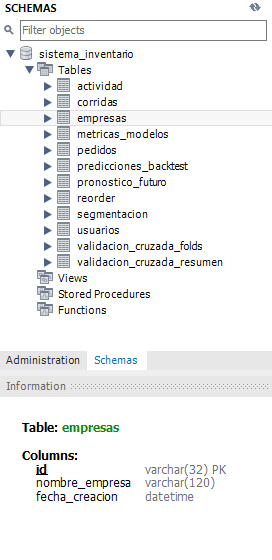
\includegraphics[height=0.35\textheight]{templatefigures/mysql_workbench_empresas}
    \caption{Estructura de la tabla \texttt{empresas} vista desde MySQL Workbench, conectado a la base de datos local.}
    \label{fig:mysql_workbench_empresas}
\end{figure}

La tabla \texttt{empresas} existe en la base de datos con las columnas descritas anteriormente: un identificador de tipo \texttt{varchar(32)} como clave primaria, el nombre de la empresa, y la fecha de creacion del registro.

\begin{figure}[H]
    \centering
    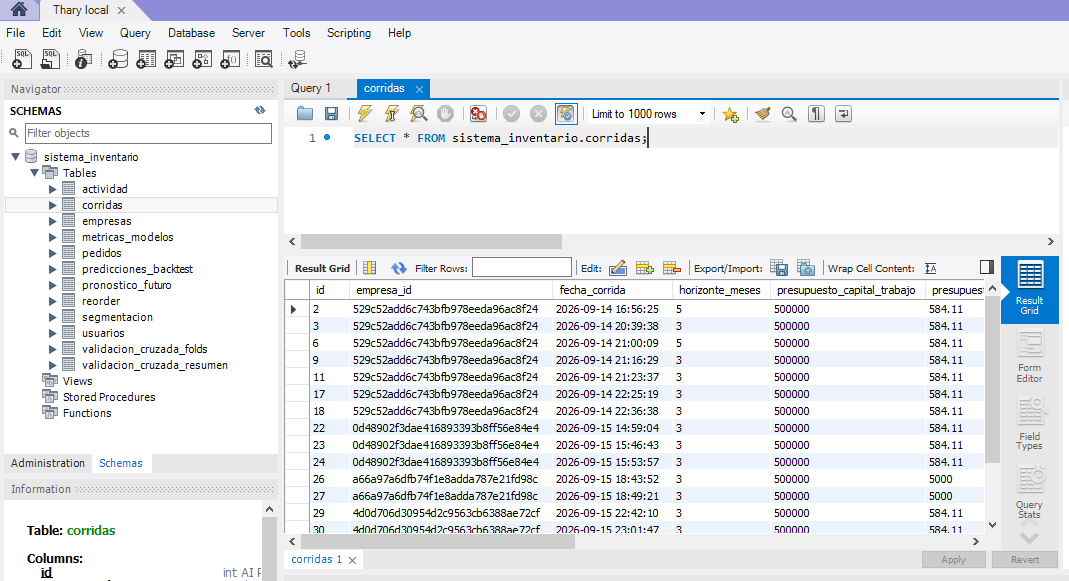
\includegraphics[height=0.3\textheight]{templatefigures/mysql_workbench_corridas}
    \caption{Consulta sobre la tabla \texttt{corridas} en MySQL Workbench, mostrando el esquema completo de 12 tablas y el historial acumulado de corridas.}
    \label{fig:mysql_workbench_corridas}
\end{figure}

La Fig. \ref{fig:mysql_workbench_corridas} muestra la confirmacion de que cada procesamiento de archivo genera una fila nueva en \texttt{corridas} sin eliminar las anteriores. Existen multiples filas asociadas a una misma empresa, correspondientes a distintas corridas realizadas en distintasfechas y horas.


\paragraph{Diseño UX/UI}
% Guia: flujos de usuario, wireframes y criterios de usabilidad y accesibilidad.
El nombre del sistema "Thary" fue elegido en la etapa de diseño de identidad visual, es un nombre corto escogido por foneticamente sonar similar a las ultimas cuatro letras de la palabra "Inventory", (inventario en ingles). En cuanto a icono representativo, se eligio la figura de un buho, para transmitir la idea de orden y control, ya que los buhos son animales reconocidos por su capacidad de percepcion y vigilancia, relacionado a como Thary se encarga de detectar señales de riesgo que podrian afectar el inventario de una empresa.

\begin{figure}[H]
    \centering
    
\includegraphics[width=0.5\textwidth]{templatefigures/logo}
    \caption{Logotipo de Thary, compuesto por el nombre del sistema y el icono representativo del búho}
    \label{fig:ux_login_logo}
\end{figure}

Para realizar el diseño de interaccion de Thary, se decidio separar las pantallas en dos: Una dirigida exclusivamente a los administradores y otra dirigida a los empleados del inventario. Al ingresar al sistema, un usuario con el rol de administrador sigue el siguiente flujo:

El usuario inicia sesion o se registra de no tener una cuenta.

\begin{figure}[H]
    \centering
    
\includegraphics[width=0.5\textwidth]{templatefigures/ux_login}
    \caption{Pantalla de inicio de sesion de Thary}
    \label{fig:ux_login}
\end{figure}

\begin{figure}[H]
    \centering
    
\includegraphics[width=0.5\textwidth]{templatefigures/ux_registro}
    \caption{Pantalla de registro de Thary}
    \label{fig:ux_registro}
\end{figure}

El administrador inicia en la pantalla de inicio del sistema, desde la cual puede acceder a la funcionalidad de carga de archivo (\textit{index}), al haber cargado el archivo correctamnete y que este sea valido, se le redirige automaticamente al dashboard, donde al seleccionar "Pronostico de demanda", se muestran los resultados.

\begin{figure}[H]
    \centering
    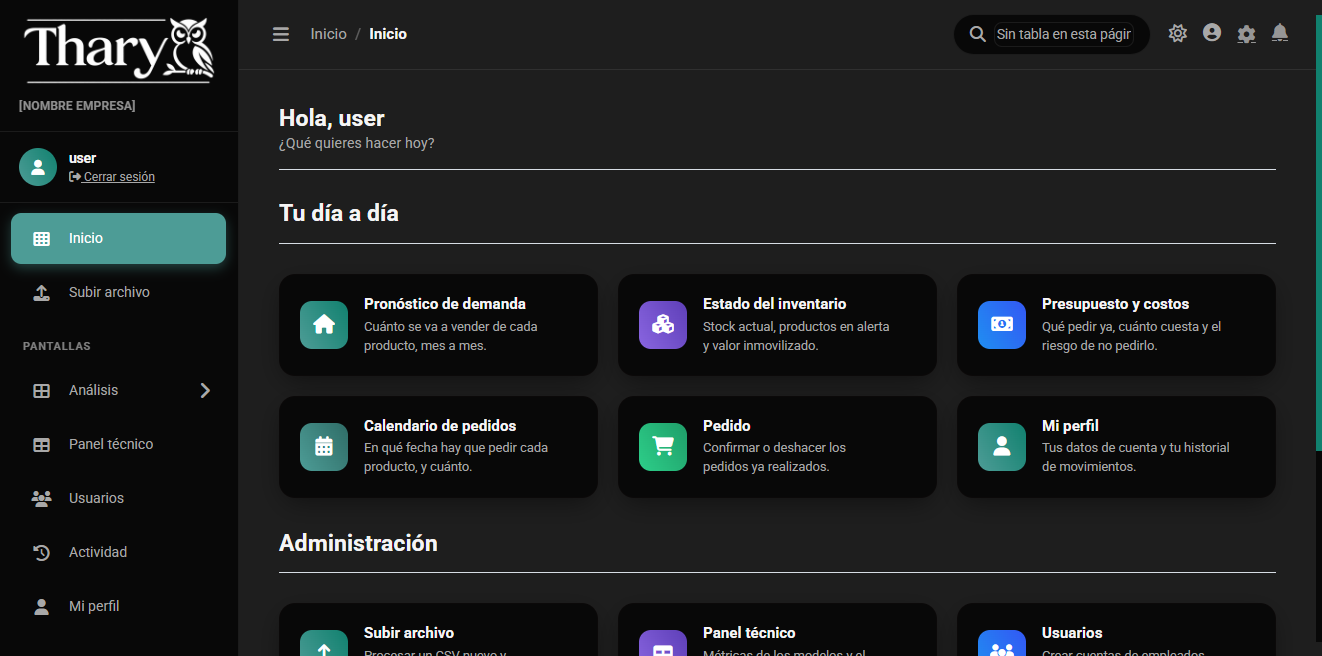
\includegraphics[width=0.5\textwidth]{templatefigures/ux_dashboard}
    \caption{Pantalla de dashboard de Thary}
    \label{fig:ux_dashboard}
\end{figure}

\begin{figure}[H]
    \centering
    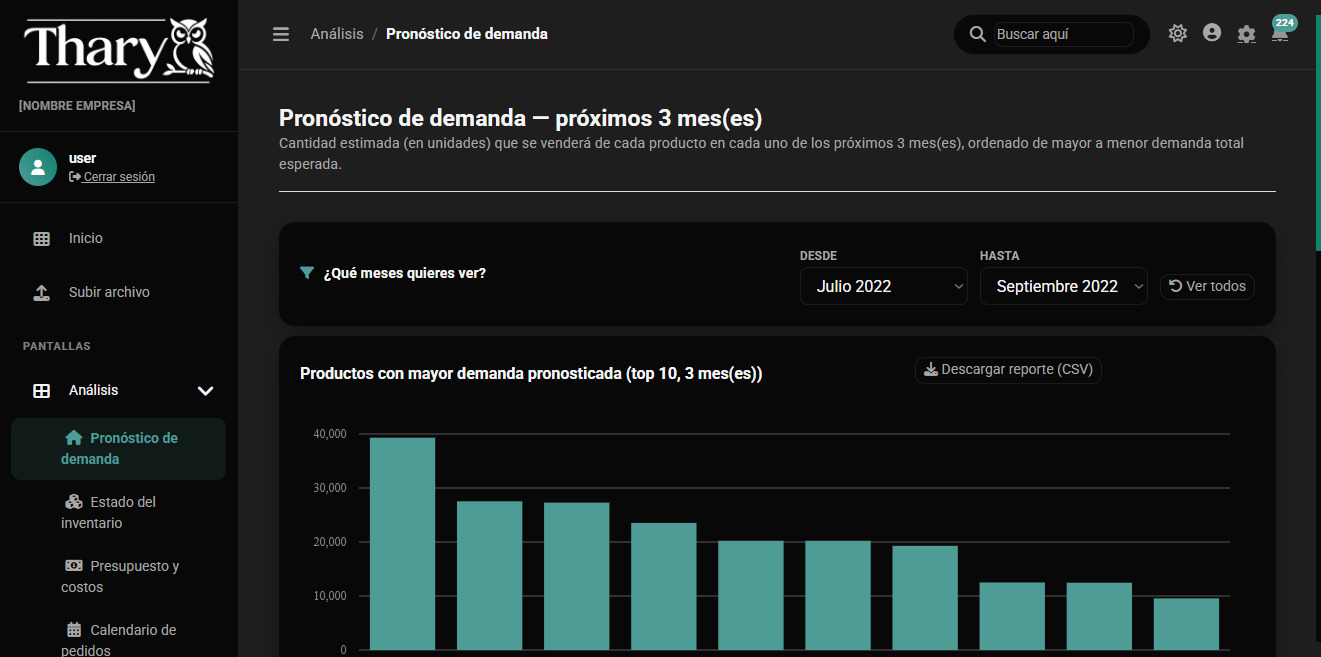
\includegraphics[width=0.5\textwidth]{templatefigures/ux_prediccion}
    \caption{Pantalla de predicción de demanda de Thary}
    \label{fig:ux_prediccion}
\end{figure}

En el sidebar, ademas de encontrar demas opciones como estado del inventario, presupuesto y pedidos, el administrador puede navegar hacia la gestion de usuarios, donde puede crear cuentas nuevas para su personal de inventario. 

\begin{figure}[H]
    \centering
    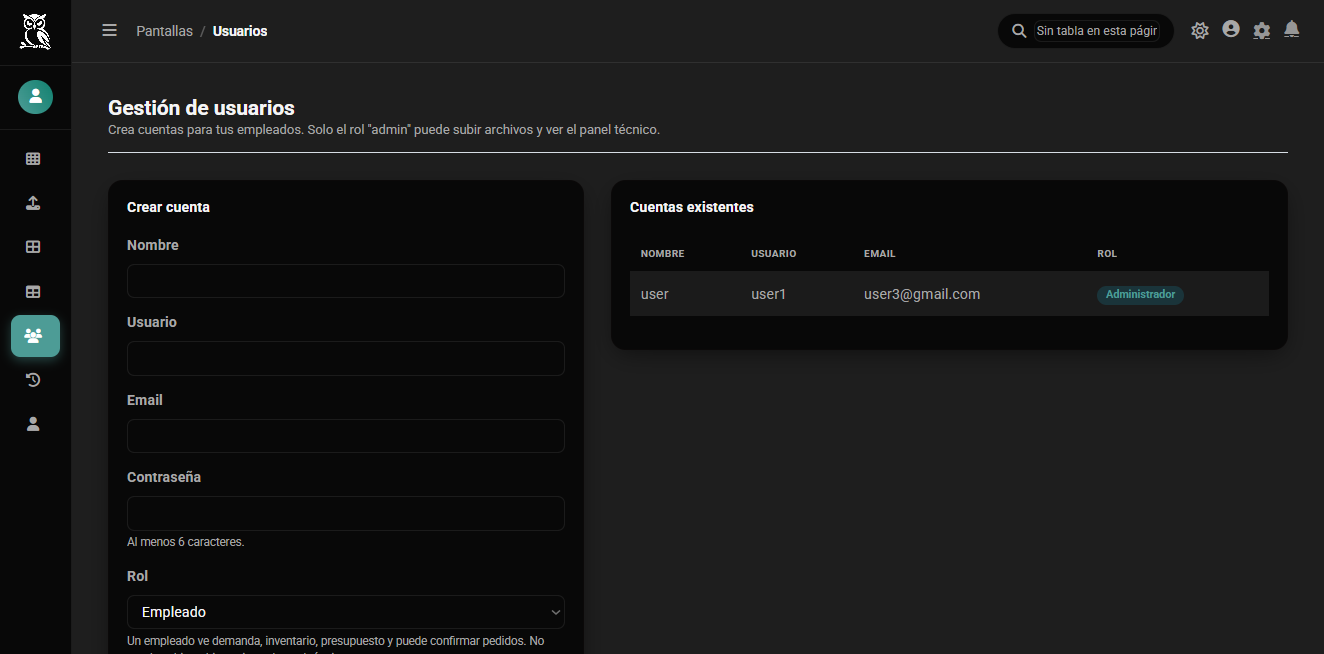
\includegraphics[width=0.5\textwidth]{templatefigures/ux_usuarios}
    \caption{Pantalla de gestión de usuarios de Thary}
    \label{fig:ux_usuarios}
\end{figure}

El flujo de los empleados es bastante similar, con la diferencia de que el perfil de un empleado cuenta con menos privilegios que el perfil de un administrador, por lo que al iniciar sesion, el empleado no puede subir ningun archivo,por lo que solo puede acceder al dashboard de la demanda pronosticada en base al csv que ya anteriormente fue cargado al sistema por el administrador que creo su cuenta, ya desde ahi, puede navegar a las mismas funcionalidades del analisis de los datos que el administrador: estado del inventario, presupuesto y pedidos. 

\begin{figure}[H]
    \centering
    \begin{subfigure}[b]{0.45\textwidth}
        \centering
        
\includegraphics[height=0.25\textheight]{templatefigures/ux_sidebar_empleado.png}
        \caption{Sidebar de empleado}
        \label{fig:ux_sidebar_empleado}
    \end{subfigure}
    \hfill
    \begin{subfigure}[b]{0.45\textwidth}
        \centering
        
\includegraphics[height=0.25\textheight]{templatefigures/ux_sidebar_administrador.png}
        \caption{Sidebar de administrador}
        \label{fig:ux_sidebar_administrador}
    \end{subfigure}
\end{figure}

\begin{figure}[H]
    \centering
    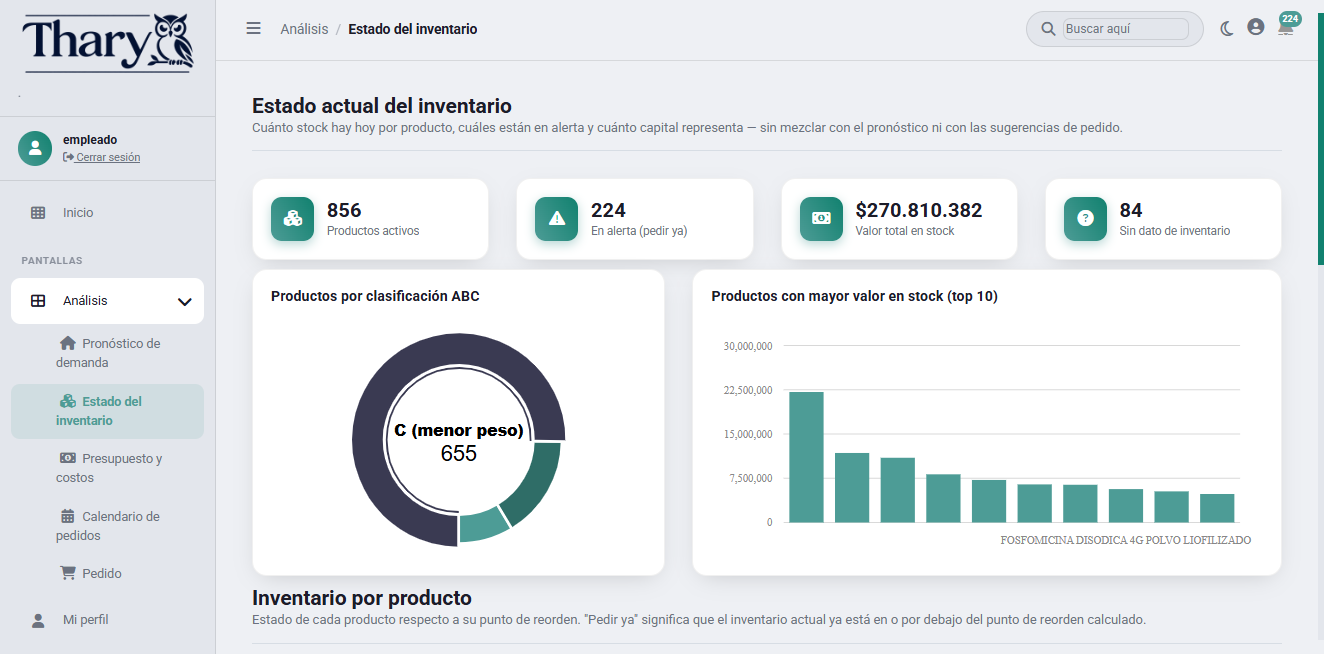
\includegraphics[height=0.25\textheight]{templatefigures/ux_estado_inventario.png}
    \caption{Estado del inventario}
    \label{fig:ux_estado_inventario}
\end{figure}

\begin{figure}[H]
    \centering
    \begin{subfigure}[b]{0.45\textwidth}
        \centering
        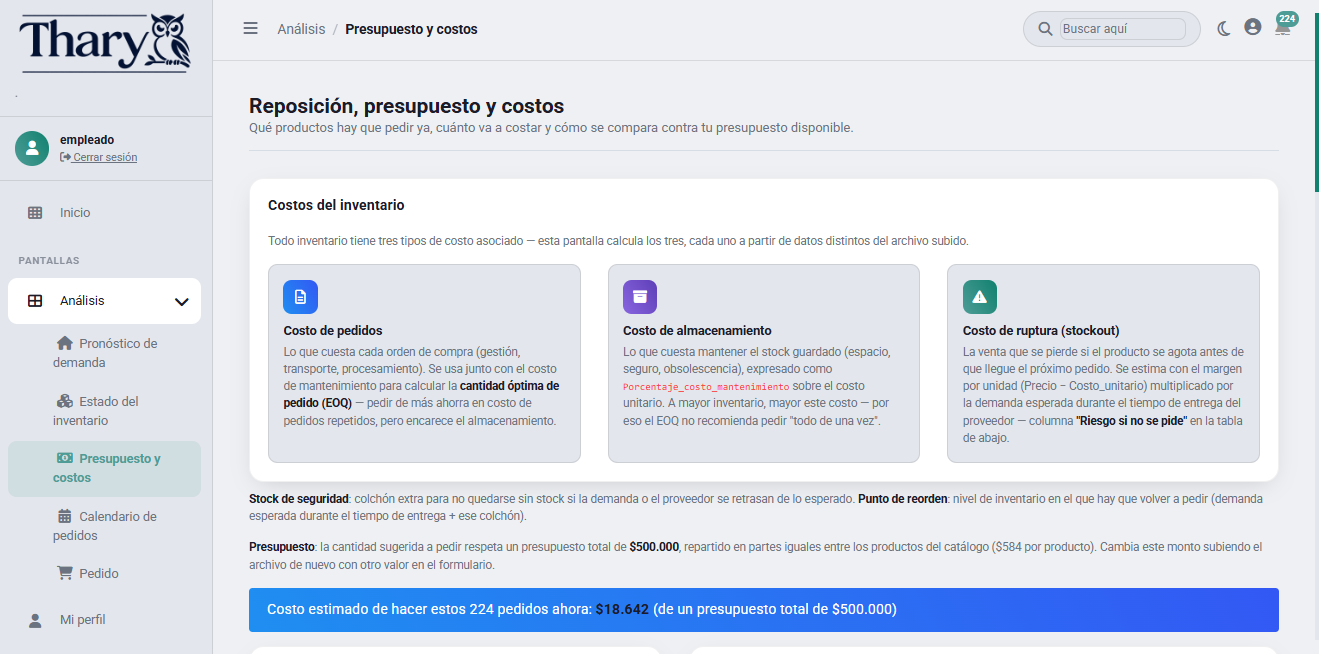
\includegraphics[height=0.25\textheight]{templatefigures/ux_presupuesto.png}
        \caption{Presupuesto}
        \label{fig:ux_presupuesto}
    \end{subfigure}
    \hfill
    \begin{subfigure}[b]{0.45\textwidth}
        \centering
        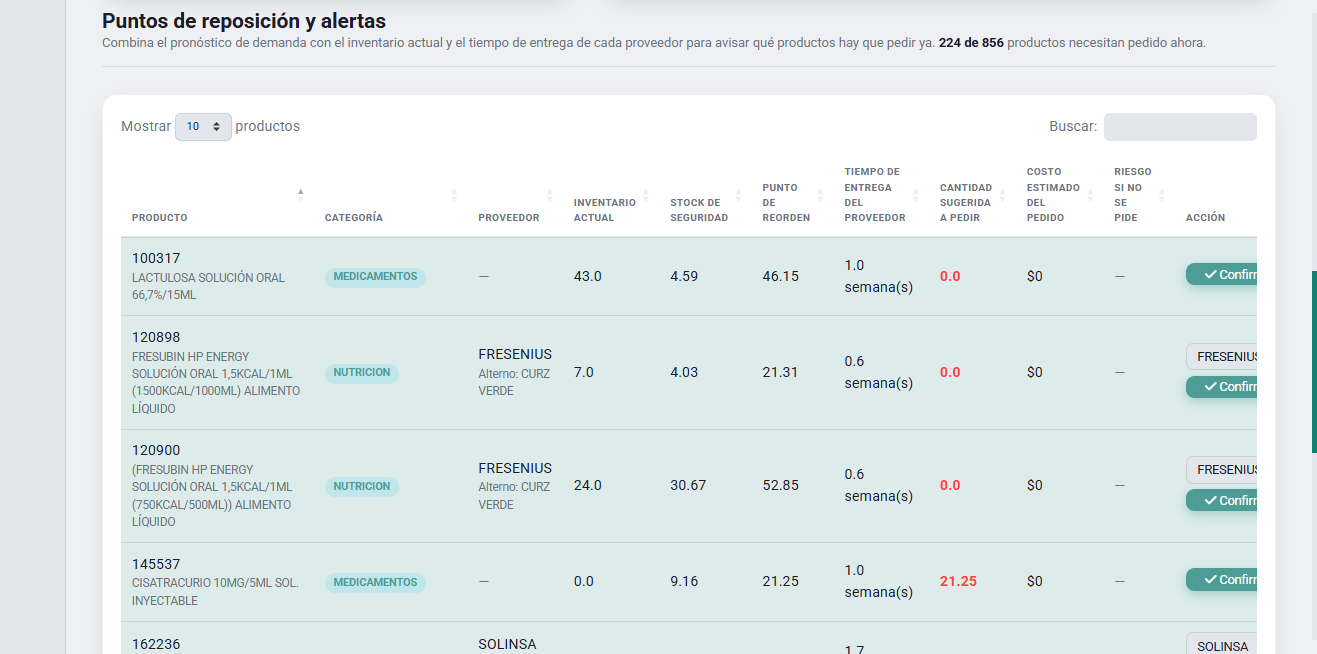
\includegraphics[height=0.25\textheight]{templatefigures/ux_reposicion_alertas.png}
        \caption{Alertas de reposición}
        \label{fig:ux_reposicion_alertas}
    \end{subfigure}
\end{figure}

La gestion de pedidos se puede ver en tres vistas: los pedidos sugeridos pendientes de confirmar, el historial de pedidos ya confirmados, y los proximos pedidos estimados segun el calendario de reposicion.

\begin{figure}[H]
    \centering
    \begin{subfigure}[b]{0.45\textwidth}
        \centering
        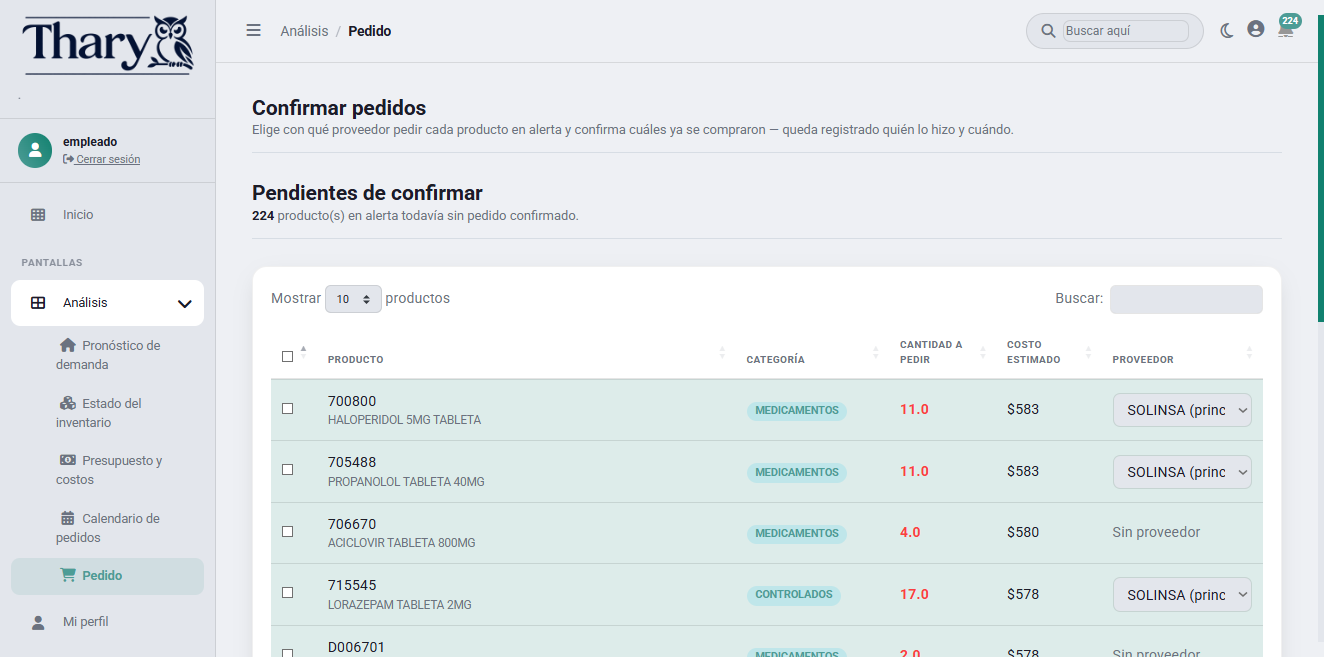
\includegraphics[height=0.25\textheight]{templatefigures/ux_pedidos.png}
        \caption{Lista de Pedidos}
        \label{fig:ux_pedidos}
    \end{subfigure}
    \hfill
    \begin{subfigure}[b]{0.45\textwidth}
        \centering
        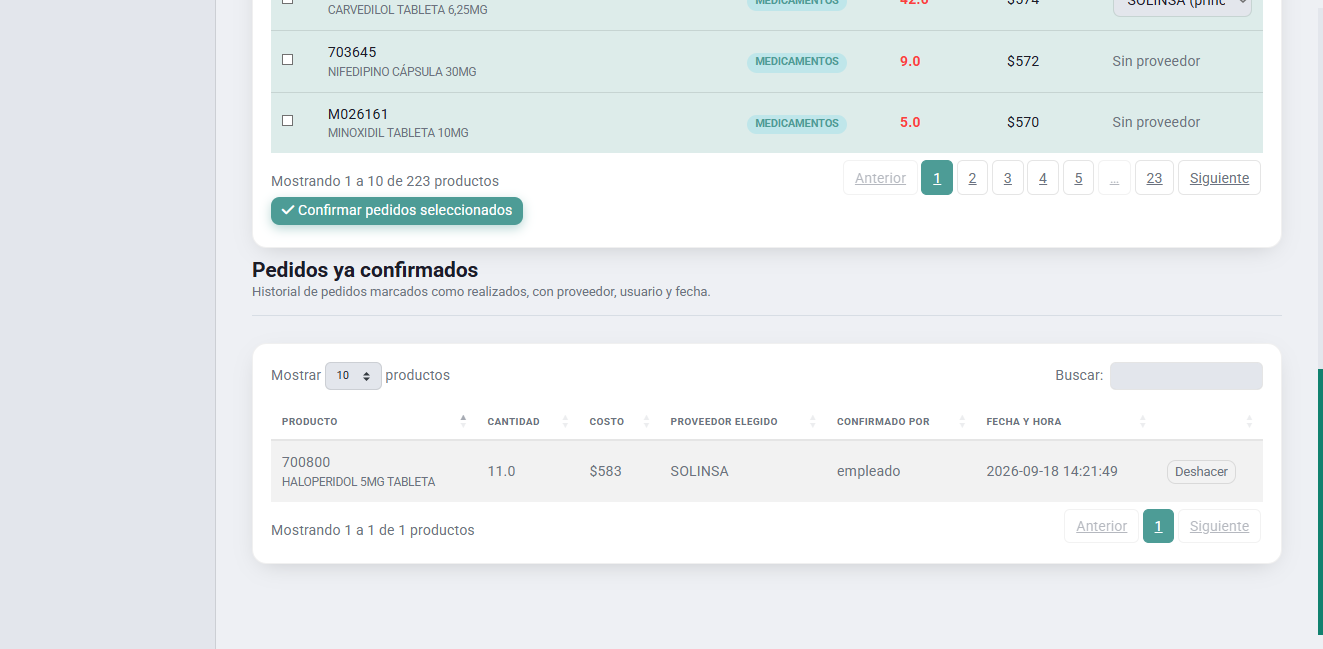
\includegraphics[height=0.25\textheight]{templatefigures/ux_pedidos_confirmados.png}
        \caption{Pedidos confirmados}
        \label{fig:ux_pedidos_confirmados}
    \end{subfigure}
\end{figure}

\begin{figure}[H]
    \centering
    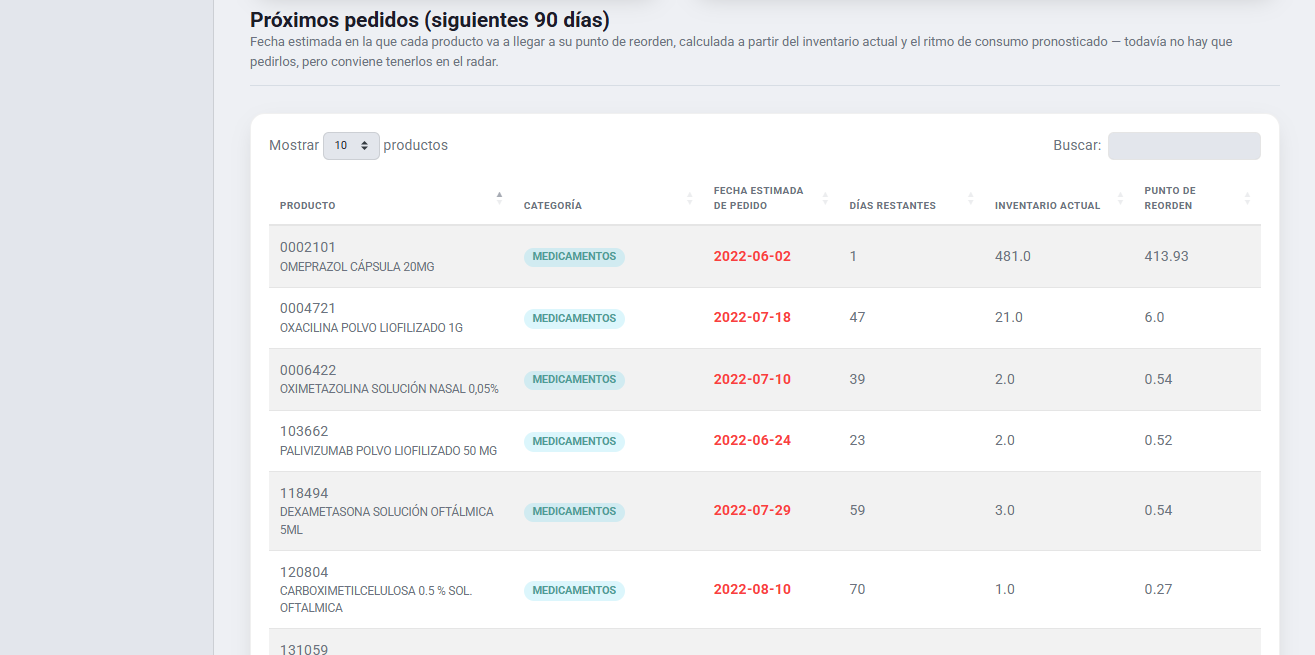
\includegraphics[height=0.25\textheight]{templatefigures/ux_prox_pedidos.png}
    \caption{Próximos pedidos}
    \label{fig:ux_prox_pedidos}
\end{figure}

\begin{figure}[H]
    \centering
    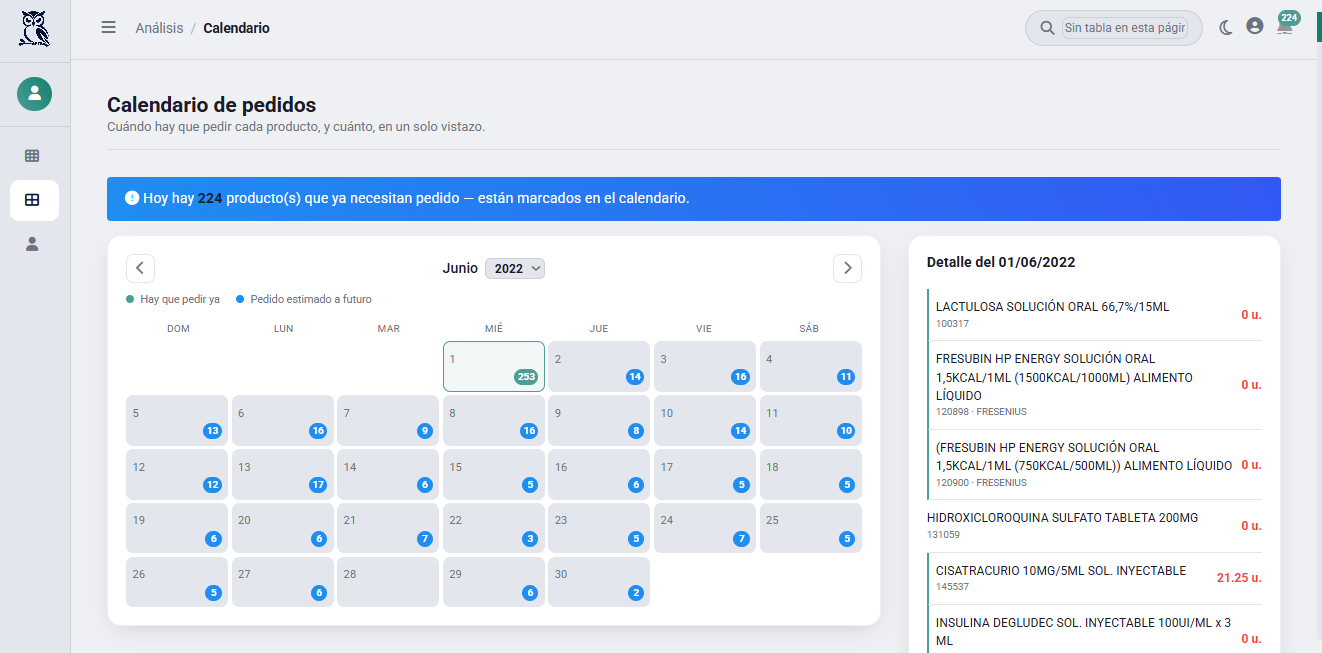
\includegraphics[height=0.25\textheight]{templatefigures/ux_calendario_pedidos.png}
    \caption{Calendario de pedidos}
    \label{fig:ux_calendario_pedidos}
\end{figure}

Una vez finalizadas sus tareas, los usuarios pueden cerrar sesion en su cuenta.

\begin{figure}[H]
    \centering
    
\includegraphics[width=0.5\textwidth]{templatefigures/ux_cerrar_sesion.png}
    \caption{Cerrar sesión}
    \label{fig:ux_cerrar_sesion}
\end{figure}

Los criterios de usabilidad que fueron tomados en cuenta fueron:

\begin{itemize}
    \item Uso de alertas visuales codificadas por color para indicar facilmente que productos se encuentran en o por debajo de su punto de reposicion y requieren ser reabastecidos inmediatamente.
    
    \begin{figure}[H]
    \centering
    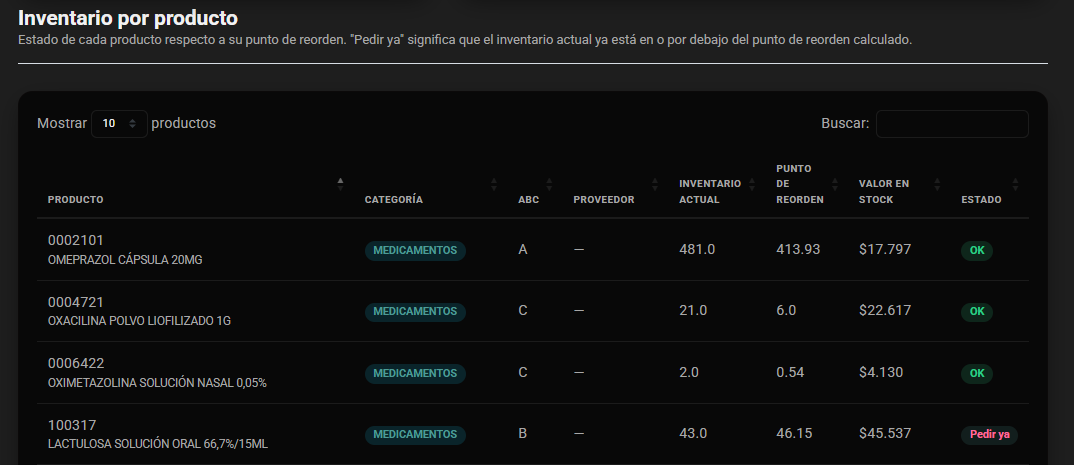
\includegraphics[width=0.5\textwidth]{templatefigures/ux_alertas_visuales.png}
    \caption{Alertas visuales}
    \label{fig:ux_alertas_visuales}
    \end{figure}

    \item Cuando un usuario con el rol de empleado inicie sesion, pero su respectivo administrador no subio ningun archivo csv, en ves de ver la pantalla del dashboard, vera una pantalla con el mensaje de que una vez el admin cargue el archivo, podra ver los analisis.

    \begin{figure}[H]
    \centering
    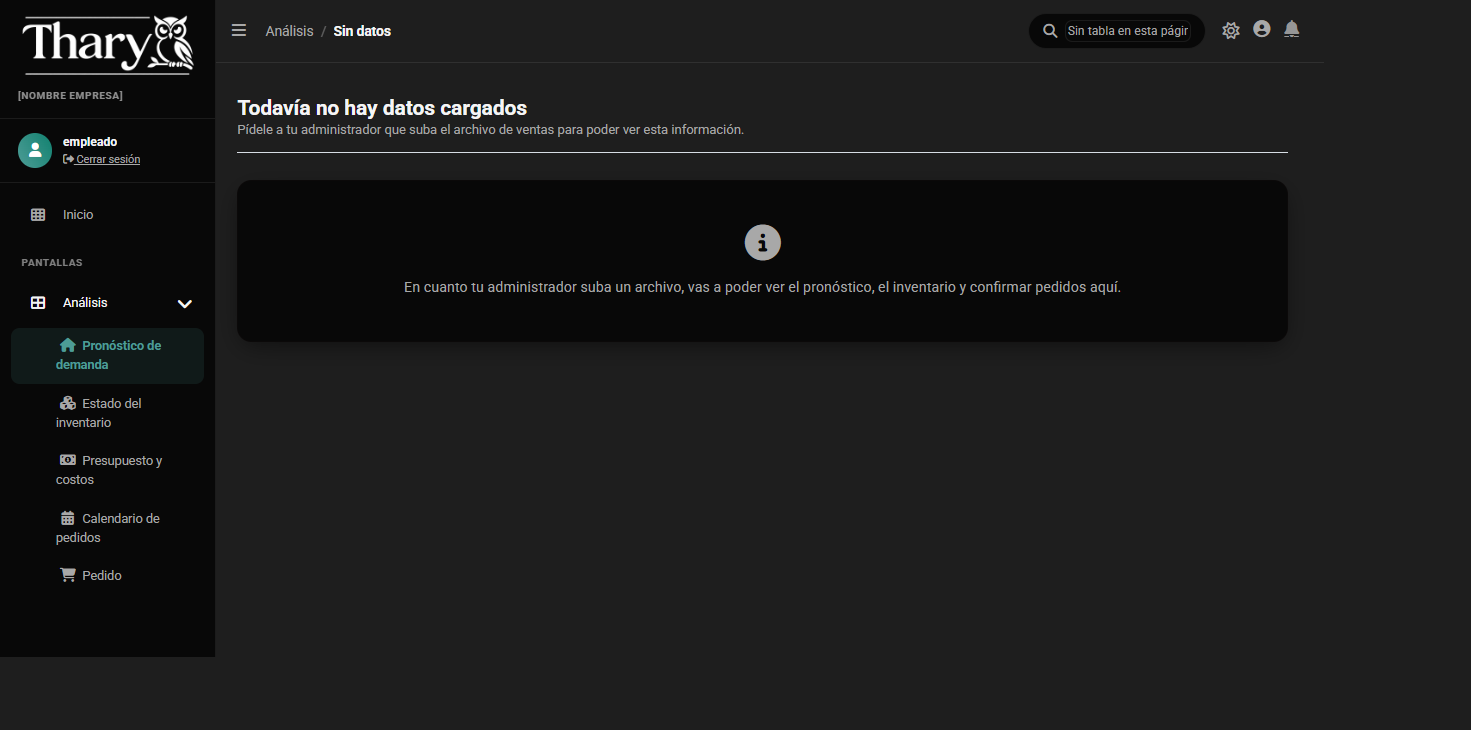
\includegraphics[width=0.5\textwidth]{templatefigures/ux_dashboard_empleado.png}
    \caption{Dashboard del empleado}
    \label{fig:ux_dashboard_empleado}
    \end{figure}
    
    \item El sistema cuenta con un modo oscuro y modo claro para que el usuario pueda escoger segun sus preferencias, mejorando la usabilidad ofreciendo ventajas como comodidad visual, menor fatiga en uso prolongado, contraste, etc.

    \begin{figure}[H]
    \centering
    
\includegraphics[width=0.5\textwidth]{templatefigures/ux_dashboard_claro.png}
    \caption{Dashboard en modo claro}
    \label{fig:ux_dashboard_claro}
    \end{figure}

    \item Thary cuenta con una version mobile, la cual le permite al usuario poder acceder a todas las funcionalidades de la version de escritorio desde su telefono movil.

        \begin{figure}[H]
    \centering
    
\includegraphics[width=0.5\textwidth]{templatefigures/ux_dashboard_mobile.png}
    \caption{Dashboard en modo mobile}
    \label{fig:ux_dashboard_mobile}
    \end{figure}
\end{itemize}

En cuanto a criterios de accesibilidad, se tomaron en cuenta los criterios de usabilidad, pero no se tomaron en cuenta mecanismos adicionales para hacer mas accesible el sistema como algun tipo de lector de pantalla para personas con discapacidad visual, o implementar un sistema de navegacion completa por teclado para alguna persona que no pueda usar un mouse. Estas falencias se reconocen como una limitacion del diseño actual, y se espera mejorarlas en el futuro. 
